\chapter*{Conclusiones}\label{cha:conclusiones}
\addcontentsline{toc}{chapter}{Conclusiones}
\markboth{Conclusiones}{Conclusiones}

\AddToShipoutPictureBG*{\put(0,0){%
        \parbox[b][\paperheight]{\paperwidth}{%
            \vfill
            \centering
            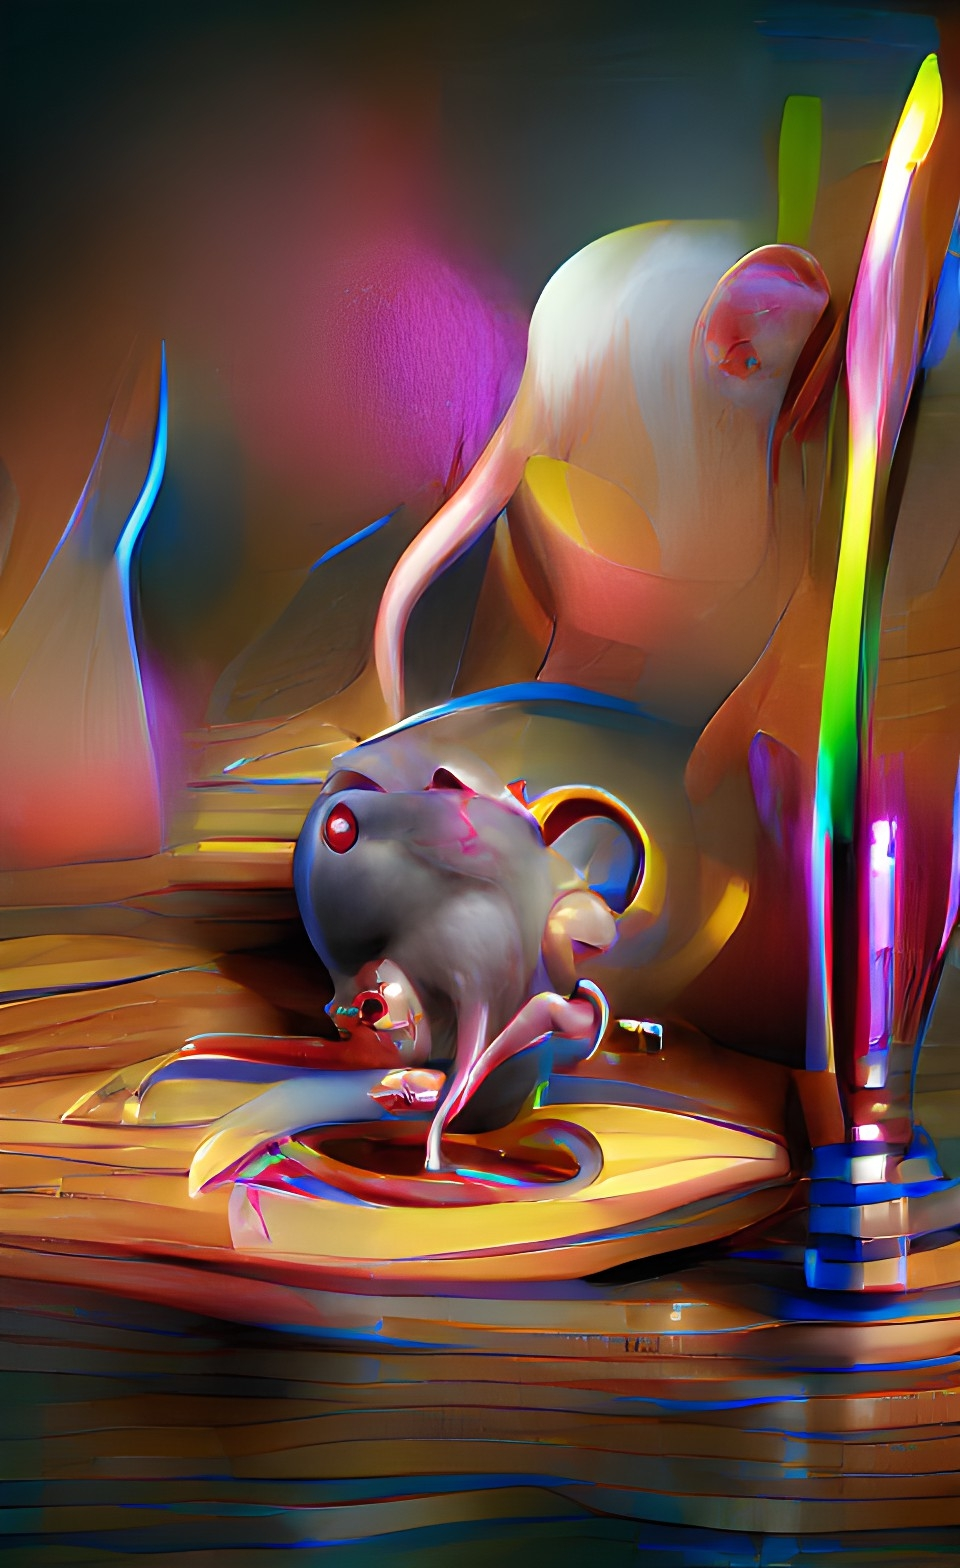
\includegraphics[width=\paperwidth,height=\paperheight,keepaspectratio]{%
                figuras/caratulas/conclusiones.jpg}\vfill
        }}}

\AddToShipoutPicture*{
    \begin{tikzpicture}[overlay, remember picture]
        \fill[white, opacity=0.75] (20, 24) rectangle (1, 22.5);
    \end{tikzpicture}}

\clearpage

Los avances tecnológicos recientes en aplicaciones del aprendizaje automático, redes neuronales artificiales profundas y técnicas de inferencia estadística son conducentes a un mejor entendimiento del comportamiento animal y de su relación con la actividad neuronal. En este trabajo hemos explorado diferentes maneras de representar el comportamiento de ratones durante su entrenamiento en la tarea rotarod con aceleración. Hemos corroborado que el algoritmo UMAP de reducción de la dimensión con segmentación \textit{watershed} es apto para la clasificación no supervisada de comportamiento animal durante la ejecución de esa tarea. A su vez, vimos que esta clasificación tiene prestaciones que son prometedoras para futuros estudios en combinación con registros de actividad neuronal. En particular, este método de análisis no supervisado permite automatizar el proceso de clasificación de comportamientos animales, brindando resultados potencialmente reproducibles entre evaluaciones y tiene la ventaja de cuantificar el comportamiento animal sin la necesidad de que intervenga manualmente un experto.

La tarea rotarod es usada tradicionalmente para evaluar impedimentos neurológicos en roedores (\autoref{cha:metodo_experimental}). Nosotros proponemos una visión renovada de esta tarea, bajo la luz de la neuroetología computacional, para analizar comportamientos descritos por múltiples características. Para que el campo de la neurociencia avance en el entendimiento de cómo el cerebro genera comportamientos ecológicamente relevantes en entornos naturales, debemos primero ser capaces de comprender las sutilezas del comportamiento animal complejo en situaciones lo más parecidas a las naturales. Esto significa estudiar el comportamiento animal sin restricciones físicas adicionales. Por desgracia, este sería un objetivo muy ambicioso de concretar. Afortunadamente, si bien la tarea rotarod presenta restricciones sobre la velocidad y el desplazamiento de los animales, constituye una excelente oportunidad para estudiar la adaptabilidad natural de sus secuencias comportamentales. En este sentido, consideramos a la tarea rotarod como una tarea natural de aprendizaje motor. Pues la manera en que los ratones adaptan su repertorio comportamental para resolver la tarea es completamente no trivial. A su vez, nuestros resultados indican que la variabilidad de estos repertorios comportamentales se reduce con el aprendizaje. También, observamos marcadas diferencias en los comportamientos de los ratones según su grado de aptitud física nato. Esta diferencia en aptitud física no se explica por su peso, sexo ni edad, aunque podría depender, por ejemplo, de su ritmo circadiano, si es que los animales son más activos en diferentes momentos del día, ya que las pruebas rotarod se realizaron por la mañana de forma regular.

El método más tradicional de representación del comportamiento, la métrica de latencia a caer, captura el progreso de los animales durante el entrenamiento y también las diferencias entre animales según su aptitud física. Adicionalmente, conseguimos definir otras métricas que describen de manera global cómo se desempeñan los ratones en la tarea, en múltiples aspectos (\autoref{cha:representacion_comportamiento}). De esta manera aportamos más información sobre el comportamiento de los ratones. Vimos que no solo aumenta la latencia a caer con el entrenamiento, sino que también aumentan la altura a la que los ratones dan pasos sobre el cilindro rotarod, mientras que la amplitud y la velocidad de los pasos se reduce. Además, registramos que las desviaciones en las ejecuciones comportamentales de los ratones se reduce con el entrenamiento. Y observamos que la mayoría de los cambios más significativos en estas métricas se dan en la segunda prueba del primer día de entrenamiento, mostrando la rapidez con la que los ratones se adaptan a nuevas situaciones. El aprendizaje motor se divide en dos fases: una fase temprana donde hay una mejora abrupta en la ejecución de la tarea, y una fase tardía donde el rendimiento mejora de manera asintótica. Curiosamente, en ambas fases participan diferentes estructuras cerebrales. Sin embargo, la latencia al caer no captura correctamente la fase tardía del aprendizaje de la tarea de rotarod. Por eso este tipo de estudios de comportamiento multidimensional permite entender las peculiaridades del aprendizaje con mayor detalle \cite{luft_motor_learning}.

Por último, hemos mostrado el potencial de esta clasificación no supervisada de poses para estudiar detalladamente la estructura temporal del comportamiento animal. En las secuencias de comportamientos, se observan marcadas preferencias por iniciar y terminar las pruebas rotarod usando determinadas categorías de comportamientos (\textit{labels}). En el \autoref{cha:mapas_comportamiento} obtuvimos dos conjuntos de \textit{labels}: uno a partir de los espectros \textit{wavelet} de partes del cuerpo de los ratones y otro a partir de características de pasos y poses adoptadas por los ratones. Observamos que los \textit{labels} de pasos y poses separan más fuertemente a los ratones según su grupo de rendimiento, comparados con los \textit{labels} \textit{wavelet}. En ambos casos, se observa que la variabilidad en las probabilidades de labels en las secuencias de comportamiento se reduce con el entrenamiento. A su vez, la entropía de las proyecciones UMAP también se reduce con los días de entrenamiento, sosteniendo que la variabilidad en las estrategias de comportamiento usadas por los ratones se reduce con el aprendizaje. El uso de mapas UMAP de dimensión reducida permite un enfoque holístico en el estudio del comportamiento: permite estudiar los efectos y cambios de múltiples características comportamentales en una conveniente representación de fácil visualización.

Esperamos que estos métodos de clasificación no supervisada de comportamiento, con algoritmos de reducción de dimensión como las proyecciones UMAP con segmentación \textit{watershed}, permitan evaluar detalladamente el desempeño físico durante la ejecución de otros tipos de tareas motoras y que también permitan cuantificar cambios a raíz de impedimentos motores como consecuencia de enfermedades neurodegenerativas. Existe evidencia experimental mostrando una reducción en la latencia a caer en modelos de la enfermedad de Parkinson y de esclerosis lateral amiotrófica \cite{costa_motor_learning, campos_parkinson}; sin embargo, estos trabajos utilizan solo la latencia a caer como métrica de rendimiento de los animales. Nosotros postulamos que el estudio detallado de los patrones de comportamiento durante la ejecución de tareas nos permitirá la detección temprana de impedimentos motores y la comparación de diferencias entre modelos experimentales de enfermedades neurodegenerativas que ayude a avanzar en la compresión de los circuitos neuronales subyacentes \cite{alfieri_motor_deficit}.

Como sucesión del trabajo desarrollado en la tesis de licenciatura, alcanzamos y superamos los objetivos propuestos hace un año y conseguimos resultados novedosos. Habíamos propuesto incorporar el uso de espectros \textit{wavelet} para capturar la dinámica del movimiento de las partes del cuerpo de los ratones. No solo hicimos eso, sino que también agregamos un segundo conjunto de características comportamentales al análisis: las características de pasos y poses. Otro de los objetivos propuestos fue estudiar el comportamiento animal durante el aprendizaje de una tarea motora. Y esto también fue alcanzado. Adicionalmente, parte del código implementado para el preprocesamiento y análisis del comportamiento animal, utilizado a lo largo de este trabajo, puede consultarse en nuestros repositorios \href{https://github.com/alvaro-concha/animal-behavior-preprocessing}{\color{blue}{animal-behavior-preprocessing}} y \href{https://github.com/alvaro-concha/animal-behavior-analysis}{\color{blue}{animal-behavior-analysis}}.